\chapter[Sobre a proposta e a metodologia]{Sobre a proposta e a metodologia}
\label{cap-sobre-a-proposta-e-a-metodologia}

\section{Ecossistemas de startups e estudos de avaliação}
\label{section:um_breve_apanhado_sobre_ecossistemas_de_startups_e_estudos_de_avaliação}

\citeonline{Schumpeter1934} diz que empreendedores tendem a se conglomerar em uma mesmo região com o objetivo de obterem benefícios mútuos, criando clusters, que podem ser interpretados como ecossistemas, e são essenciais para o desenvolvimento local. Para \citeonline{James1953} e \citeonline{Dalcin2015} empreendedores influenciam diretamente o crescimento econômico, a oferta de empregos, a redução da pobreza e a formação e o crescimento de cidades, \citeonline{Spigel2015} afirma ainda que estudos sobre ecossistemas empreendedores se tornaram uma ferramenta importante para o estudo do empreendedorismo de alto crescimento sob o ponto de vista geográfico por esta capacidade de influenciar o desenvolvimento econômico e social de uma determinada região.

Segundo \citeonline{Dubini1989} ecossistemas são marcados pela presença de empresas, economia diversificada, boa infraestrutura de negócios e investimentos, cultura empreendedora adequada e políticas públicas que apoiem o empreendedorismo e os empreendedores. \citeonline{ranga2013triple} trás o conceito da Hélice Tripla representando ecossistemas por meio da interação entre governo, indústria e universidade.

Para \citeonline{isenberg2011introducing} um ecossistema empreendedor possui seis grandes pilares: política, finanças, cultura, suporte, capital humano e mercado, onde todos devem agir em conjunto para a criação de um ecossistema saudável e promissor, essa visão está representada na Figura \ref{figure:isenberg_ecosystem} (e adaptada para o português por \citeonline{Arruda2013}. \citeonline{schwab2015} defende que os pilares de um ecossistema são abertura de mercados, capital humano, investimento, apoio do governo, ambiente regulatório, educação, universidades e suporte cultural.

\begin{figure}[!htb]
\centering
\includegraphics[width=11cm,angle=0]{figuras/isenberg_ecosystem_ptbr}
\caption{Ecossistemas empreendedores, por \citeonline{isenberg2011introducing}}
\label{figure:isenberg_ecosystem}
\end{figure}

\citeonline{gumpert1985heart} diz que enquanto governo e academia são capazes de criar condições favoráveis para que o empreendedorismo prospere o envolvimento de indivíduos, como os empreendedores, é essencial, reforçando o modelo criado por Isenberg e indo de encontro ao modelo de Hélice Quadrupla definido por \citeonline{leydesdorff2012triple}. \citeonline{carayannis2009mode} reforça ainda a importância de considerarmos mídia e cultura como variáveis que compõem essa quarta vertente que representa a sociedade civil em um ecossistema de inovação.

Nesta linha, \citeonline{Spigel2015} define ecossistemas como a união entre elementos culturais, sociais, políticos e econômicos em uma região que, juntos, propíciam o surgimento, e o crescimento, de empresas inovadoras e encorajam novos empreendedores e demais atores a assumirem os riscos relacionados a inovação. \citeonline{Suresh2012} já concentrou seus estudos em mapear os elementos de um ecossistema que contribuem para a formação do indivíduo empreendedor, como a presença de redes que os apoiem nos momentos difíceis e sirva de exemplo para os mesmos como referências de sucesso. 

\citeonline{Motoyama2014} identificaram quatro pontos de conexões cruciais que devem acontecer para o desenvolvimento de um ecossistema: conexões entre empreendedores, conexões entre organizações de suporte, conexões entre empreendedores e organizações de suporte e conexões de suporte diversas, como eventos. Esses conceitos foram de extrema importância para este trabalho.

Reforçando a relevância das conexões em um ecossistema \citeonline{Hwang2012} fala sobre a importância dos indivíduos ``keystone'' por serem os responsáveis por quebrar barreiras sociais ``invisíveis'' que são impostas entre os diferentes atores de um ecossistema, como entre novos empreendedores e possíveis investidores ou parceiros. Os autores relatam ainda que quanto mais facilmente essas barreiras são quebradas em um determinado ecossistema mais frutífero ele será.

\citeonline{Stangler2015}, por meio da Kauffman Foundation, definem as quatro seguintes características de um ecossistema vibrante: densidade, fluídez, conectividade e diversidade. Por densidade entendem questões como a quantidade de novas empresas para cada mil habitantes, a quantidade de postos de trabalho da região e o tamanho dos setores que envolvam alta tecnologia. Para fluídez indicam questões como o fluxo populacional de uma cidade, a realocação no mercado de trabalho e a quantidade de empresas de alto crescimento. Para conectividade os indicadores podem ser relacionados a redes de investidores, conectividade entre programas e a quantidade de spin-offs, como são chamadas as empresas que foram criadas por pessoas relacionadas a outras empresas mais antigas e estabelecidas, geralmente criadas por ex-funcionários. Por fim, diversidade idealmente pode ser entendida como a quantidade de especializações econômicas na região, a taxa de mobilidade social e dados relativos a imigração. O artigo em si não descreve um arcabouço para avaliação de ecossistemas, mas define bons indicadores que podem ser utilizados por outros trabalhos.

\citeonline{Feld2012} desenvolveu a ``Teoria de Boulder'' a qual ele define quatro regras para um ecossistema de qualidade: 1) Precisa ser liderado por empreendedores; 2) Os líderes precisam assumir um compromisso a longo prazo para com o ecossistema; 3) O ecossistema precisa ser inclusivo para qualquer pessoa que queira participar; e 4) O ecossistema precisa ter atividades contínuas que engajem a comunidade empreendedora local. Ele também elencou alguns atores que compõem e são de grande importância para ecossistemas como empreendedores, governo, universidades, investidores, mentores, provedores de serviços e grandes empresas já estabelecidas localmente. Outro fator interessante é que o autor enxerga ecossistemas empreendedores como organismos vivos em constante evolução, e não estruturas bem definidas e estáticas. Com base nesse princípio ele também faz a divisão de atores entre ``semeadores'' (seeders, aqueles que fomentam e contribuem para o crescimento do ecossistema) e ``consumidores'' (feeders, todos aqueles que não atuam como semeadores e se beneficiam com o crescimento do ecossistema).  

Partindo para a avaliação de ecossistemas os pesquisadores \citeonline{Arnaud2009} e \citeonline{Ahmad2007} apresentaram metodologias centradas em três grandes pilares: 1) Fatores determinantes, envolvendo indicadores de ambiente regulatório, acesso a capital, cultura e capacidades empreendedoras; 2) Performance, englobando indicadores relativos ao desenvolvimento das empresas da região; e 3) Impacto, envolvendo indicadores sociais como índices de geração de empregos, crescimento econômico e redução da pobreza.

Com base nos pilares definidos por \citeonline{Arnaud2009} o pesquisador brasileiro \citeonline{Arruda2013} desenvolveu um estudo sobre o ecossistema de startups brasileiro, como resultados obtiveram visões sobre o modelo regulatório brasileiro, as nossas condições de mercado, o acesso a financiamento, a criação e a difusão de conhecimento, a capacidade e a cultura empreendedora e demais peculiaridades regionais do Brasil. O trabalho também lista em anexo todas as variáveis mapeadas para o trabalho e suas fontes, que foram de grande importância para este trabalho. Nas recomendações de trabalho futuro mencionam a dificuldade em conversar sobre experiências de fracasso com os empreendedores brasileiros, em especial com aqueles que ainda não obtiveram algum caso de sucesso, talvez esse problema se repita no contexto do Distrito Federal e pode ser interpretado como reflexo de imaturidade no ecossistema. A metodologia utilizada por Arruda se assemelha a deste trabalho por se tratar de uma abordagem mista (quantitativa e qualitativa) e ter como base entrevistas com atores relevantes para o ecossistema.

\citeonline{Hermann2015}, por meio do ``The Global Startup Ecosystem Ranking'' e da ``Compass'', realizaram um estudo sobre ecossistemas com base em seis pilares principais: performance, financiamento, alcance de mercado, talento, experiência em startups e índice de crescimento. 

\citeonline{Kutt2013}, por meio de uma análise quantitativa de diversas bases de dados locais e globais fez uma comparação do ecossistema de startups da Estônia em um contexto internacional, comparando-o como Finlândia, Taiwan, Israel, Coreia e Singapura. O autor também fez um estudo por meio da análise de dados de redes sociais para obter uma visualização das estruturas sociais do ecossistema da Estônia e identificar como os atores se conectam entre si. Essa metodologia também se aproxima da forma como este trabalho fora abordado.

A \citeonline{indiceglobaldoempreendedorismo} publica anualmente o Índice de Cidades Empreendedoras e tem sua análise de ecossistemas baseada em sete pilares: ambiente regulatório, infraestrutura, mercado, acesso a capital, inovação, capital humano e cultura empreendedora. De acordo com os índices de 2015 e 2016 Brasília demonstrou uma melhora significativa em alguns dos pilares mas, também, piora em outras, como demonstrado pela Figura \ref{figure:ici20152016}. 

\begin{figure}[!htb]
	\centering
	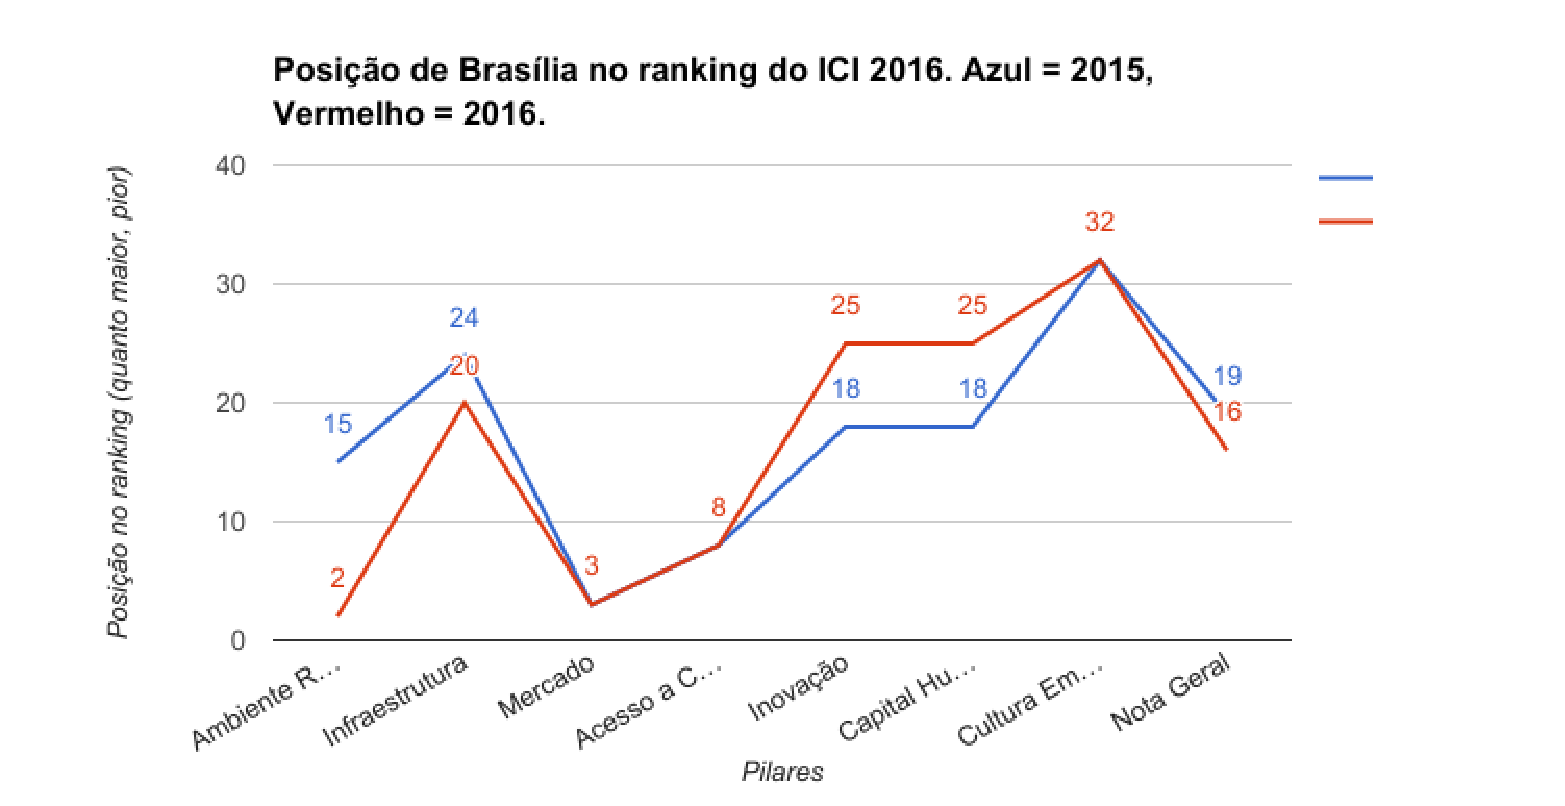
\includegraphics[width=11cm,angle=0]{figuras/ici20152016}
	\caption{Indicadores de Brasília no Índice de Cidades Empreendedoras}
	\label{figure:ici20152016}
\end{figure}

O primeiro indicador exibido na Figura \ref{figure:ici20152016} representa o Ambiente Regulatório do Distrito Federal, o saldo da 15a posição para a 2a entre 32 cidades analisadas deu-se por melhorias no rito burocrático para abertura de empresas de baixo-risco, como startups, desde as mudanças tornou-se possível abrir uma empresa em aproximadamente 7 dias por meio de um processo totalmente online. O segundo, de Infraestrutura, tem como base dados referentes ao transporte interurbano e condições urbanas, como \% da população com acesso a internet, fluidez do trânsito, taxa de homícidios, custo médio da energia elétrica e preço médio do metro quadrado. O DF peca, principalmente, no transporte interurbano e no alto custo de vida. Em seguida temos o indicador de Mercado, destaque para o Distrito Federal graças a sua forte renda per capta. Nos três indicadores seguintes, Inovação, Capital Humano e Capital Empreendedora, o DF demonstra seus piores indicadores, reflexo de poucos incentivos ao empreendedorismo, ciência, tecnologia e inovação.